\begin{figure}
	\tikzsetnextfilename{succ-triangolo}
	\centering
	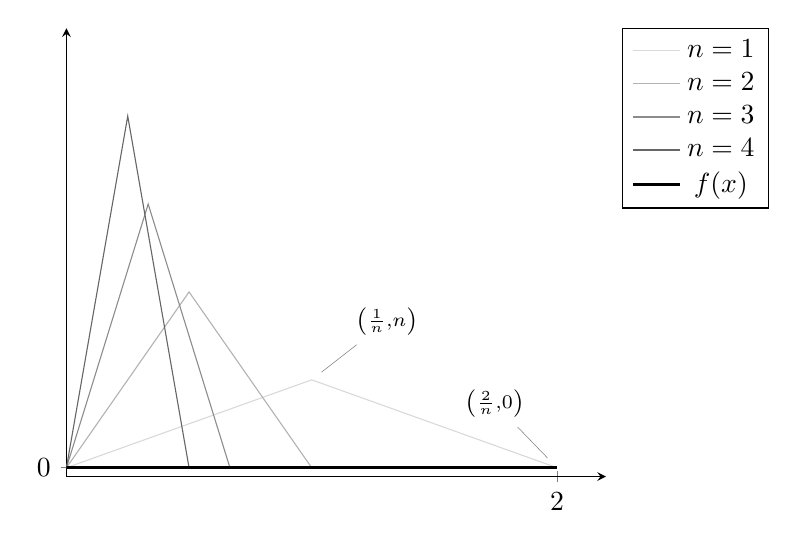
\begin{tikzpicture}
		\begin{axis}[
						enlargelimits,
						legend pos=outer north east,
						axis x line=bottom,axis y line=middle,
						xmin=0,xmax=2.2,ymin=-0.1,ymax=5,ytick={0},xtick={2}
					]
			\addplot [color=black!15!white] coordinates {(0,0) (1/1,1) (2/1,0)};
			\addplot [color=black!30!white] coordinates {(0,0) (1/2,2) (2/2,0)};
			\addplot [color=black!45!white] coordinates {(0,0) (1/3,3) (2/3,0)};
			\addplot [color=black!60!white] coordinates {(0,0) (1/4,4) (2/4,0)};
			\addplot [very thick,color=black,domain=0:2]  {0};
			\node [pin=45:{$\scriptstyle\left(\frac1{n},n\right)$}] at (axis cs:1,1) {};
			\node [pin=120:{$\scriptstyle\left(\frac2{n},0\right)$}] at (axis cs:2,0) {};
			\legend{$n=1$,$n=2$,$n=3$,$n=4$,$f(x)$}
		\end{axis}
	\end{tikzpicture}
	\caption{La successione dell'esempio 3, in $[0,2]$, forma un triangolo di area 1 con l'asse delle ascisse, indipendentemente dal valore di $n$. L'altezza del triangolo aumenta infinitamente al crescere di $n$, mentre la base tende a zero.}
	\label{fig:succ_triangolo}
\end{figure}
